% ===================================
% CODICE LaTeX PER GRAFICI E TABELLE
% Tesi GDO - Capitoli 1 e 2
% ===================================
% filepath: c:\Users\saint\tesi\nuovi grafi 1 e 2.tex
\documentclass[12pt,a4paper]{article}
% Pacchetti necessari
\usepackage[utf8]{inputenc}
\usepackage[T1]{fontenc}
\usepackage{amsmath}
\usepackage{amssymb}    
\usepackage{graphicx}
\usepackage{caption}
\usepackage{subcaption} % Per sottotitoli nelle figure
% Preambolo necessario:
\usepackage{tikz}
\usepackage{pgfplots}
\usepackage{booktabs}
\usepackage{multirow}
\pgfplotsset{compat=1.17}
\usetikzlibrary{pgfplots.polar}

% ===================================
% CAPITOLO 1
% ===================================
\begin{document}
% FIGURA 1.1: Gap tra Ricerca e Implementazione
\begin{figure}[h]
\centering
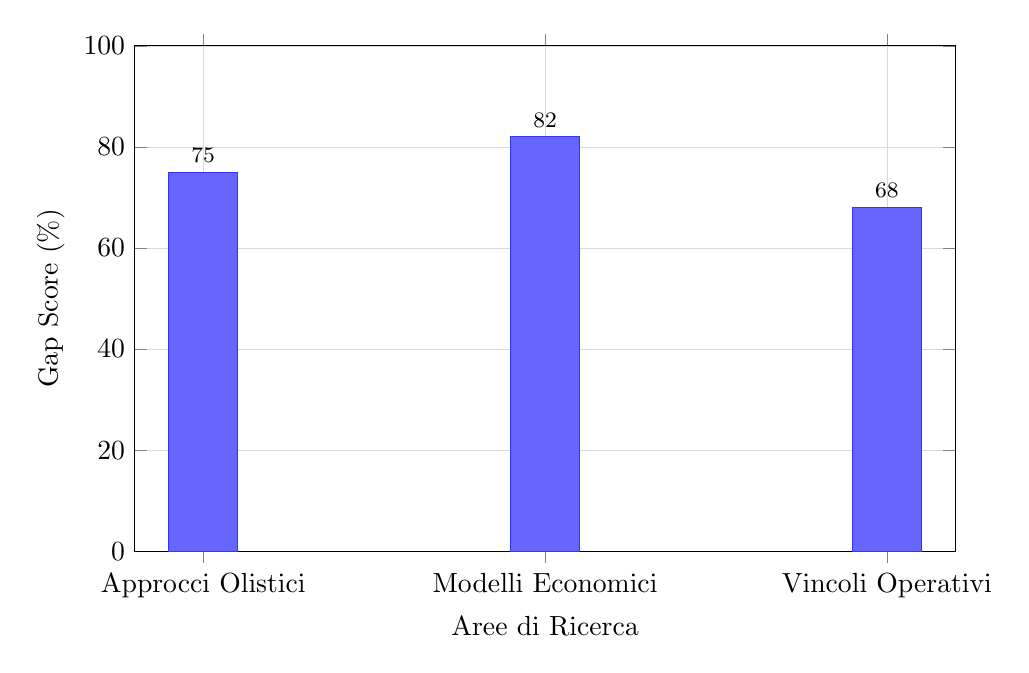
\begin{tikzpicture}
\begin{axis}[
    ybar,
    width=12cm,
    height=8cm,
    ylabel={Gap Score (\%)},
    xlabel={Aree di Ricerca},
    symbolic x coords={Approcci Olistici,Modelli Economici,Vincoli Operativi},
    xtick=data,
    ymin=0,
    ymax=100,
    bar width=25pt,
    nodes near coords,
    every node near coord/.append style={font=\footnotesize},
    grid=major,
    grid style={line width=.1pt, draw=gray!30},
    legend style={at={(0.5,-0.15)},anchor=north}
]
\addplot[fill=blue!60, draw=blue!80] coordinates {
    (Approcci Olistici,75)
    (Modelli Economici,82)
    (Vincoli Operativi,68)
};
\end{axis}
\end{tikzpicture}
\caption{Gap identificati tra ricerca accademica e implementazione pratica nella GDO}
\label{fig:gap_ricerca}
\end{figure}

% FIGURA 1.2: Framework GIST - Architettura Concettuale
\begin{figure}[h]
\centering
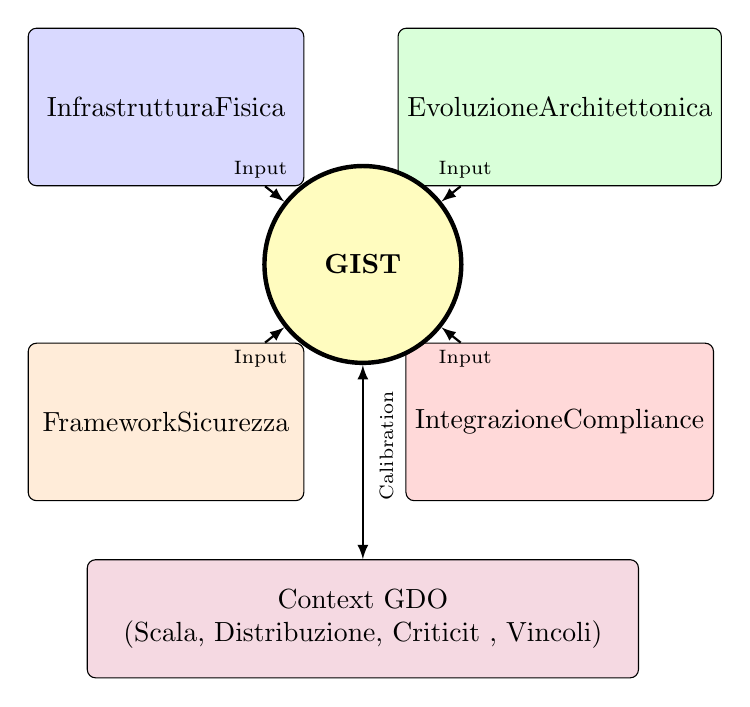
\begin{tikzpicture}[
    box/.style={rectangle, draw, text centered, minimum width=3.5cm, minimum height=2cm, rounded corners=3pt},
    contextbox/.style={rectangle, draw, text centered, minimum width=7cm, minimum height=1.5cm, rounded corners=3pt},
    arrow/.style={->, thick, >=latex},
    node distance=3.5cm
]

% Componenti principali
\node[box, fill=blue!15] (physical) at (0,0) {Infrastruttura\newline Fisica};
\node[box, fill=green!15] (arch) at (5,0) {Evoluzione\newline Architettonica};
\node[box, fill=orange!15] (security) at (0,-4) {Framework\newline Sicurezza};
\node[box, fill=red!15] (compliance) at (5,-4) {Integrazione\newline Compliance};

% Framework centrale GIST
\node[circle, draw, fill=yellow!25, minimum size=2.5cm, ultra thick] (gist) at (2.5,-2) {\textbf{GIST}};

% Context GDO
\node[contextbox, fill=purple!15, align=center] (context) at (2.5,-6.5) {Context GDO\\(Scala, Distribuzione, Criticit , Vincoli)};

% Connessioni
\draw[arrow] (physical) -- (gist);
\draw[arrow] (arch) -- (gist);
\draw[arrow] (security) -- (gist);
\draw[arrow] (compliance) -- (gist);
\draw[arrow, <->] (gist) -- (context);

% Etichette delle connessioni
\node[font=\scriptsize] at (1.2,-0.8) {Input};
\node[font=\scriptsize] at (3.8,-0.8) {Input};
\node[font=\scriptsize] at (1.2,-3.2) {Input};
\node[font=\scriptsize] at (3.8,-3.2) {Input};
\node[font=\scriptsize, rotate=90] at (2.8,-4.3) {Calibration};

\end{tikzpicture}
\caption{Architettura concettuale del Framework GIST (GDO Integrated Security Transformation)}
\label{fig:gist_framework}
\end{figure}

% FIGURA 1.3: Decomposizione del Framework GIST
\begin{figure}[h]
\centering
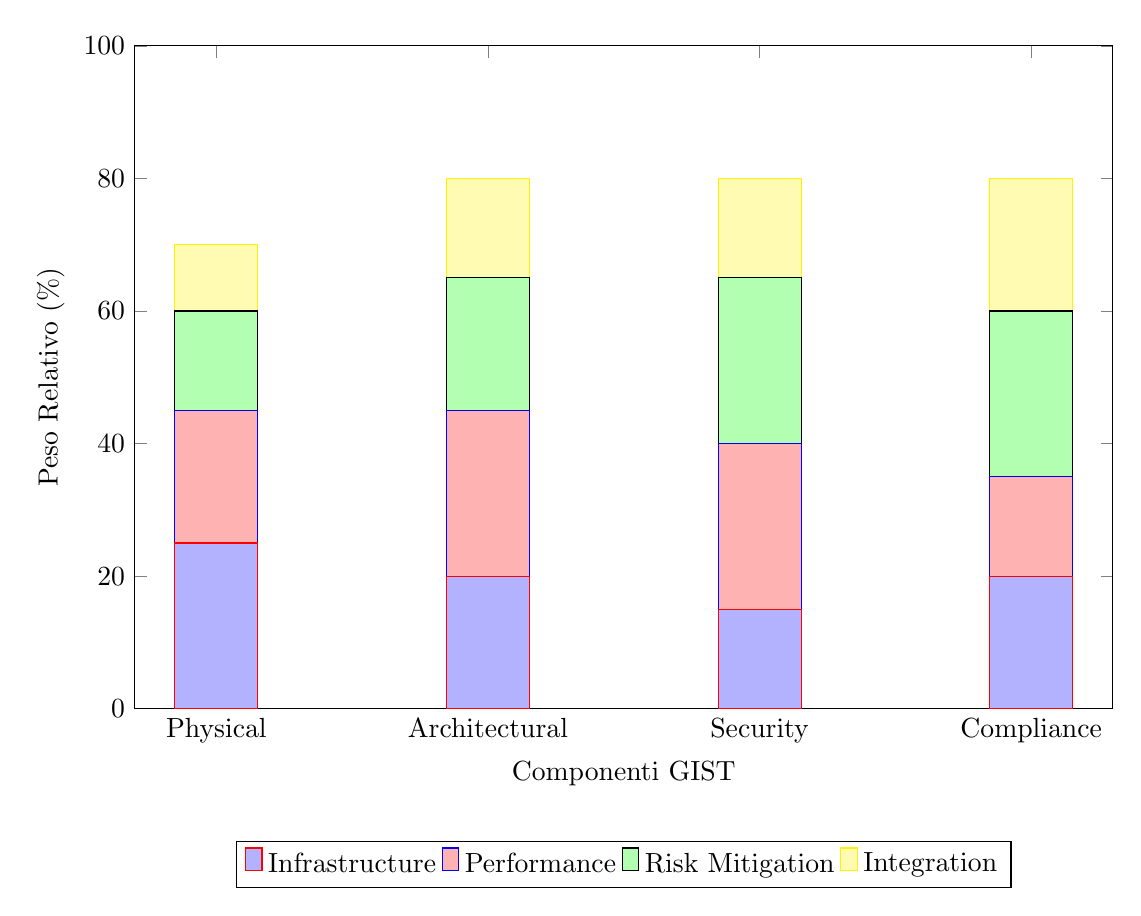
\begin{tikzpicture}
\begin{axis}[
    width=14cm,
    height=10cm,
    ybar stacked,
    ylabel={Peso Relativo (\%)},
    xlabel={Componenti GIST},
    symbolic x coords={Physical,Architectural,Security,Compliance},
    xtick=data,
    ymin=0,
    ymax=100,
    bar width=30pt,
    legend style={at={(0.5,-0.2)},anchor=north,legend columns=4},
    cycle list name=color list
]
\addplot+[ybar,fill=blue!30] coordinates {(Physical,25) (Architectural,20) (Security,15) (Compliance,20)};
\addplot+[ybar,fill=red!30] coordinates {(Physical,20) (Architectural,25) (Security,25) (Compliance,15)};
\addplot+[ybar,fill=green!30] coordinates {(Physical,15) (Architectural,20) (Security,25) (Compliance,25)};
\addplot+[ybar,fill=yellow!30] coordinates {(Physical,10) (Architectural,15) (Security,15) (Compliance,20)};

\legend{Infrastructure,Performance,Risk Mitigation,Integration}
\end{axis}
\end{tikzpicture}
\caption{Decomposizione dei pesi relativi nel Framework GIST per diversi scenari operativi}
\label{fig:gist_decomposition}
\end{figure}

% ===================================
% CAPITOLO 2
% ===================================

% TABELLA 2.1: Metriche di Evoluzione degli Attacchi POS
\begin{table}[h]
\centering
\caption{Metriche di evoluzione degli attacchi POS 2019-2025}
\label{tab:evoluzione_attacchi}
\begin{tabular}{lccccc}
\toprule
\textbf{Periodo} & \textbf{n Campioni} & \textbf{Success Rate (\%)} & \textbf{Detection Rate (\%)} & \textbf{Persistenza (giorni)} & \textbf{p-value} \\
\midrule
2019-2021 & 89 & $73.0 \pm 4.2$ & $85.4 \pm 3.1$ & $14.3 \pm 2.1$ & $<0.001$ \\
2022-2023 & 76 & $45.1 \pm 5.3$ & $62.7 \pm 4.8$ & $23.7 \pm 3.4$ & $<0.001$ \\
2024-2025 & 69 & $61.8 \pm 4.7$ & $33.9 \pm 5.9$ & $41.2 \pm 5.2$ & $<0.001$ \\
\bottomrule
\multicolumn{6}{l}{\scriptsize Test $\chi^2$: $\chi^2(4)=67.82$, $p<0.001$ (differenze significative tra periodi)}
\end{tabular}
\end{table}

% FIGURA 2.1: Modello Tridimensionale dei Fattori di Vulnerabilità
\begin{figure}[h]
\centering
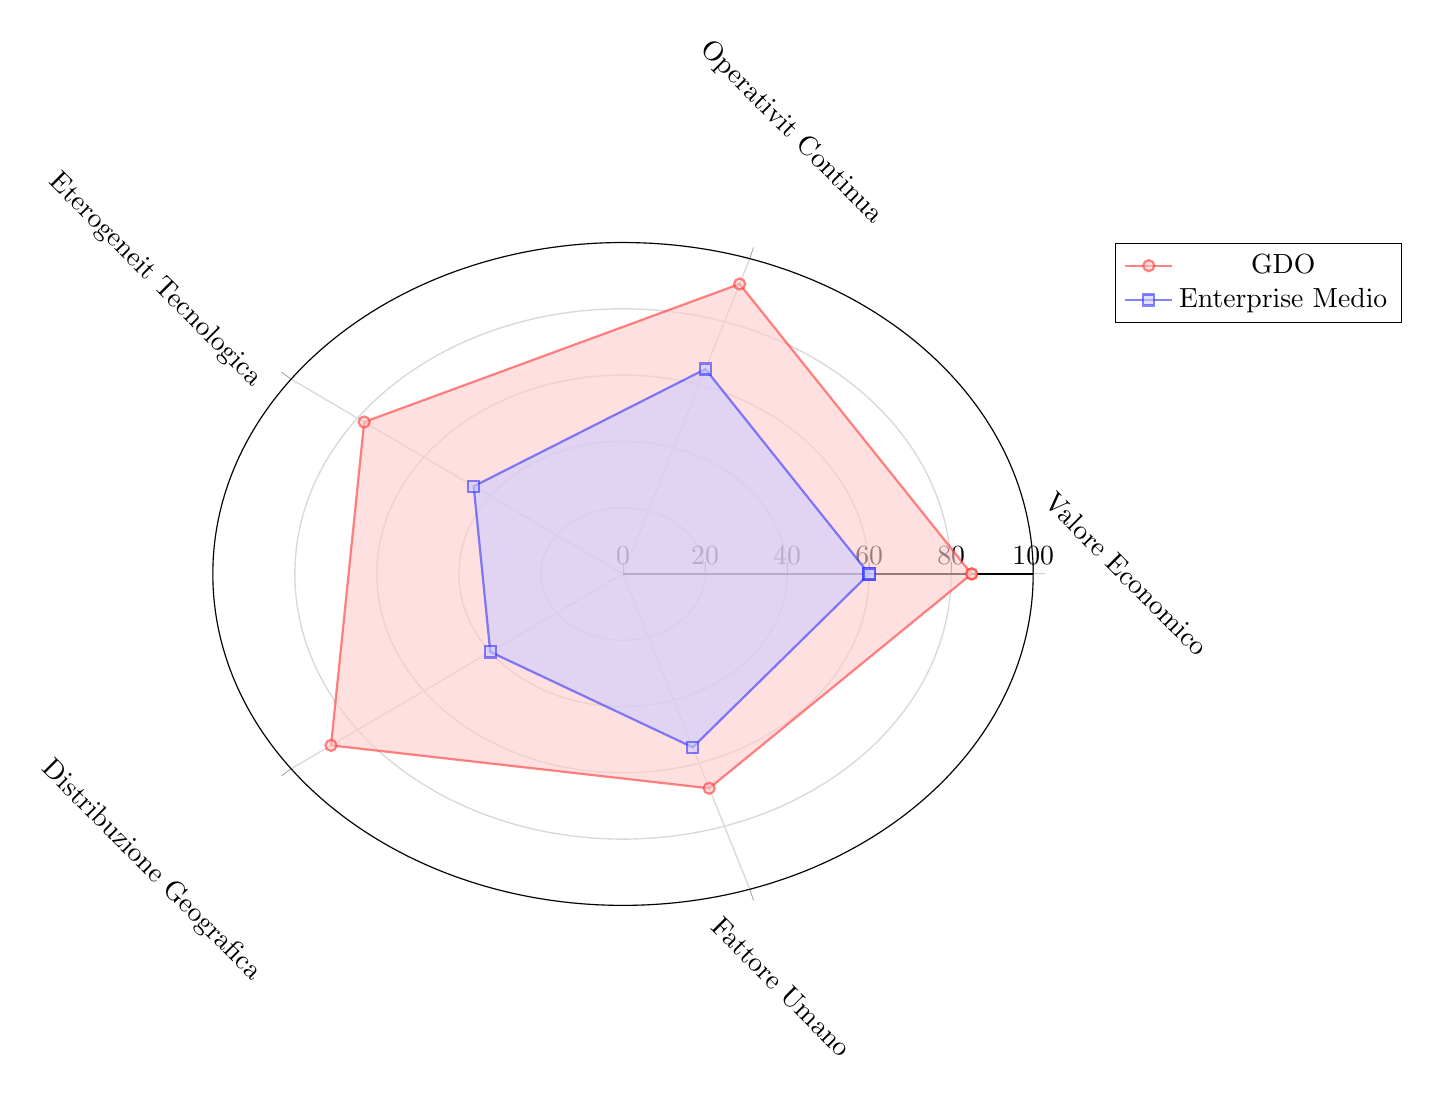
\begin{tikzpicture}
\begin{polaraxis}[
    width=12cm,
    height=10cm,
    xlabel style={font=\footnotesize},
    ylabel style={font=\footnotesize},
    xtick={0,72,144,216,288},
    xticklabels={
        \rotatebox{-45}{Valore Economico},
        \rotatebox{-45}{Operativit  Continua},
        \rotatebox{-45}{Eterogeneit  Tecnologica},
        \rotatebox{-45}{Distribuzione Geografica},
        \rotatebox{-45}{Fattore Umano}
    },
    ytick={0,20,40,60,80,100},
    ymin=0,
    ymax=100,
    grid=both,
    grid style={line width=0.5pt, draw=gray!30},
    legend style={at={(1.1,1)},anchor=north west}
]
\addplot[thick,mark=*,red!80,fill=red!20,opacity=0.6] coordinates {
    (0,85) (72,92) (144,78) (216,88) (288,68) (360,85)
};
\addlegendentry{GDO}

\addplot[thick,mark=square*,blue!80,fill=blue!20,opacity=0.6] coordinates {
    (0,60) (72,65) (144,45) (216,40) (288,55) (360,60)
};
\addlegendentry{Enterprise Medio}
\end{polaraxis}
\end{tikzpicture}
\caption{Modello tridimensionale dei fattori di vulnerabilit  - Confronto GDO vs Enterprise}
\label{fig:vulnerabilita_3d}
\end{figure}

% FIGURA 2.2: Curva di Propagazione del Malware
\begin{figure}[h]
\centering
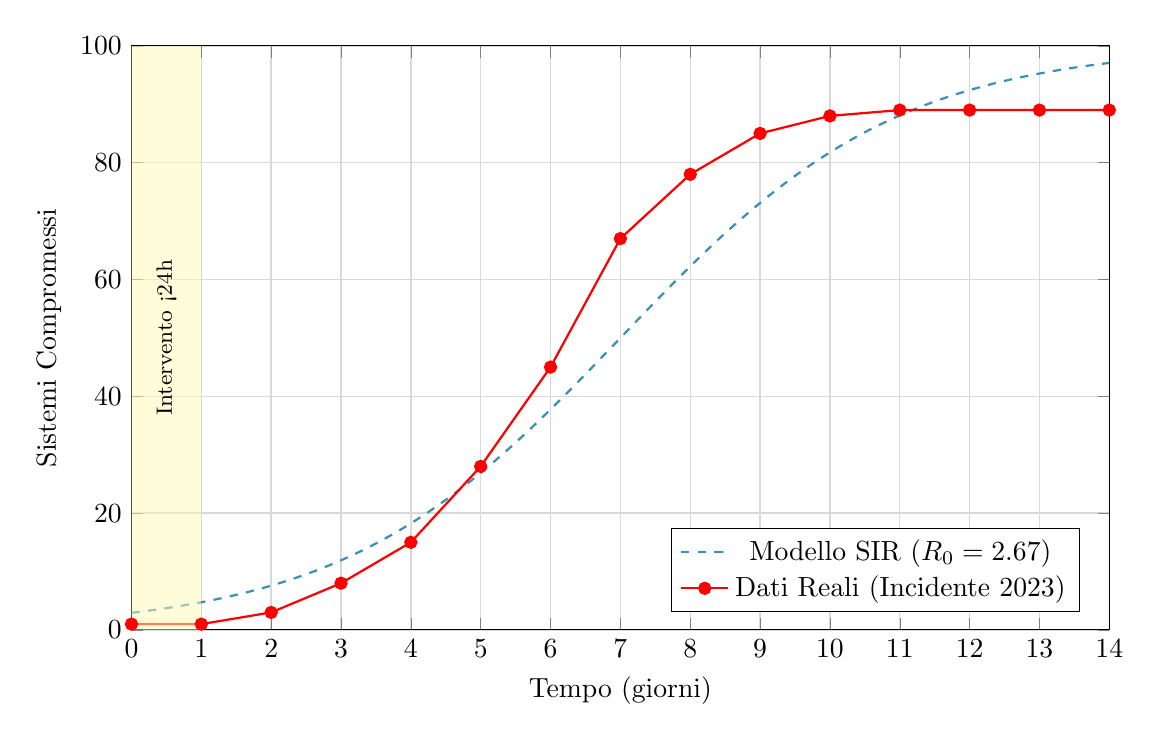
\begin{tikzpicture}
\begin{axis}[
    width=14cm,
    height=9cm,
    xlabel={Tempo (giorni)},
    ylabel={Sistemi Compromessi},
    xmin=0,
    xmax=14,
    ymin=0,
    ymax=100,
    grid=major,
    grid style={line width=0.5pt, draw=gray!30},
    legend pos=south east
]

% Modello SIR teorico
\addplot[
    domain=0:14,
    samples=100,
    smooth,
    thick,
    dashed,
    cyan!70!black
] {100/(1 + exp(-0.5*(x-7)))};
\addlegendentry{Modello SIR ($R_0 = 2.67$)}

% Dati reali
\addplot[
    thick,
    mark=*,
    red
] coordinates {
    (0,1) (1,1) (2,3) (3,8) (4,15) (5,28) 
    (6,45) (7,67) (8,78) (9,85) (10,88) 
    (11,89) (12,89) (13,89) (14,89)
};
\addlegendentry{Dati Reali (Incidente 2023)}

% Area di intervento ottimale
\fill[yellow!30,opacity=0.5] (0,0) rectangle (1,100);
\node[rotate=90] at (0.5,50) {\footnotesize Intervento <24h};

\end{axis}
\end{tikzpicture}
\caption{Curva di propagazione del malware: confronto tra modello SIR e dati reali dell'incidente 2023}
\label{fig:propagazione_malware}
\end{figure}

% FIGURA 2.3: Decomposizione STL
\begin{figure}[h]
\centering
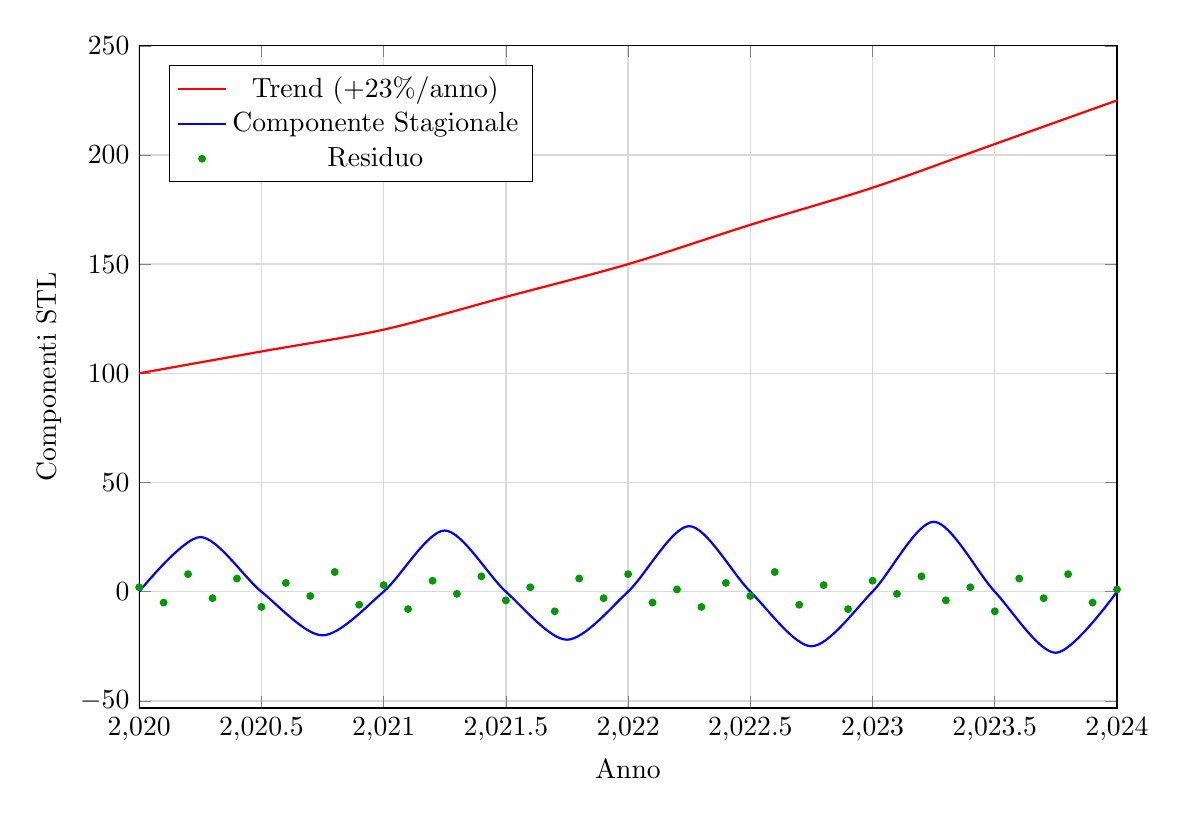
\begin{tikzpicture}
\begin{axis}[
    width=14cm,
    height=10cm,
    xlabel={Anno},
    ylabel={Componenti STL},
    xmin=2020,
    xmax=2024,
    legend pos=north west,
    grid=major,
    grid style={line width=0.5pt, draw=gray!30}
]

% Trend
\addplot[thick,red,smooth] table[x=year,y=trend] {
year trend
2020.0 100
2020.5 110
2021.0 120
2021.5 135
2022.0 150
2022.5 168
2023.0 185
2023.5 205
2024.0 225
};
\addlegendentry{Trend (+23\%/anno)}

% Stagionalità
\addplot[thick,blue,smooth] table[x=year,y=seasonal] {
year seasonal
2020.0 0
2020.25 25
2020.5 0
2020.75 -20
2021.0 0
2021.25 28
2021.5 0
2021.75 -22
2022.0 0
2022.25 30
2022.5 0
2022.75 -25
2023.0 0
2023.25 32
2023.5 0
2023.75 -28
2024.0 0
};
\addlegendentry{Componente Stagionale}

% Residuo
\addplot[thick,green!60!black,only marks,mark size=1pt] table[x=year,y=residual] {
year residual
2020.0 2
2020.1 -5
2020.2 8
2020.3 -3
2020.4 6
2020.5 -7
2020.6 4
2020.7 -2
2020.8 9
2020.9 -6
2021.0 3
2021.1 -8
2021.2 5
2021.3 -1
2021.4 7
2021.5 -4
2021.6 2
2021.7 -9
2021.8 6
2021.9 -3
2022.0 8
2022.1 -5
2022.2 1
2022.3 -7
2022.4 4
2022.5 -2
2022.6 9
2022.7 -6
2022.8 3
2022.9 -8
2023.0 5
2023.1 -1
2023.2 7
2023.3 -4
2023.4 2
2023.5 -9
2023.6 6
2023.7 -3
2023.8 8
2023.9 -5
2024.0 1
};
\addlegendentry{Residuo}

\end{axis}
\end{tikzpicture}
\caption{Decomposizione STL degli attacchi GDO 2020-2024}
\label{fig:stl_decomposition}
\end{figure}

% FIGURA 2.4: Confronto Costi Compliance
\begin{figure}[h]
\centering
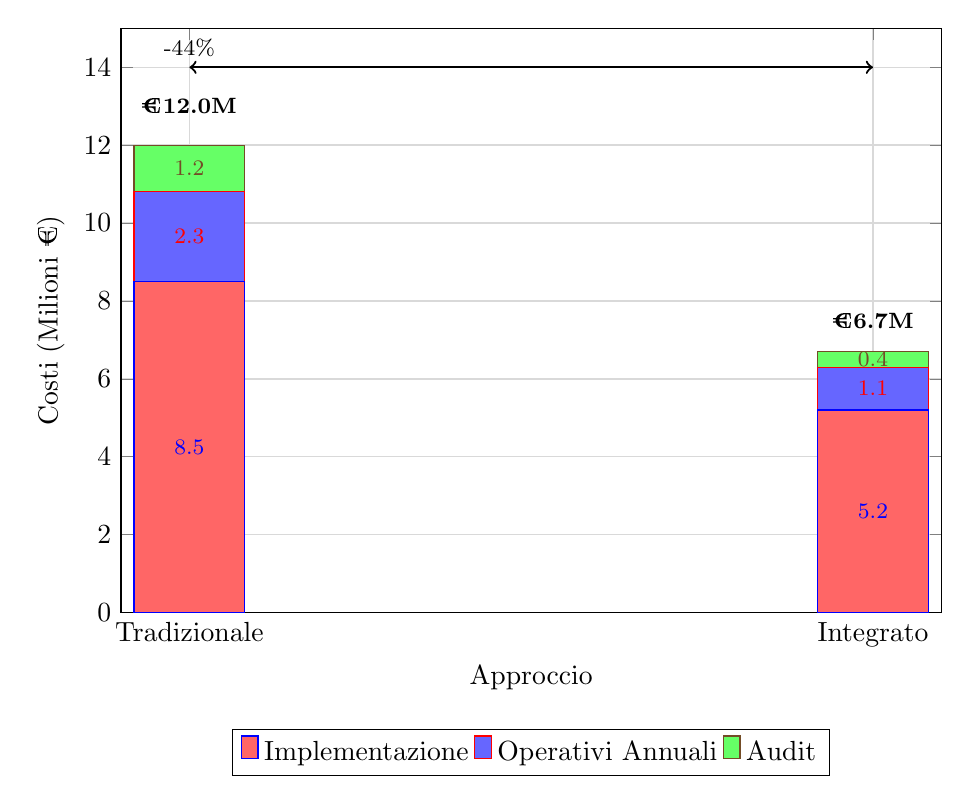
\begin{tikzpicture}
\begin{axis}[
    ybar stacked,
    width=12cm,
    height=9cm,
    ylabel={Costi (Milioni €)},
    xlabel={Approccio},
    symbolic x coords={Tradizionale,Integrato},
    xtick=data,
    bar width=40pt,
    ymin=0,
    ymax=15,
    legend style={at={(0.5,-0.2)},anchor=north,legend columns=3},
    nodes near coords,
    every node near coord/.append style={font=\footnotesize},
    grid=major,
    grid style={line width=0.5pt, draw=gray!30}
]

\addplot+[ybar,fill=red!60] coordinates {(Tradizionale,8.5) (Integrato,5.2)};
\addplot+[ybar,fill=blue!60] coordinates {(Tradizionale,2.3) (Integrato,1.1)};
\addplot+[ybar,fill=green!60] coordinates {(Tradizionale,1.2) (Integrato,0.4)};

\legend{Implementazione,Operativi Annuali,Audit}

% Etichette totali
\node at (axis cs:Tradizionale,13) {\footnotesize \textbf{€12.0M}};
\node at (axis cs:Integrato,7.5) {\footnotesize \textbf{€6.7M}};

% Risparmio percentuale
\draw[<->,thick] (axis cs:Tradizionale,14) -- (axis cs:Integrato,14);
\node at (axis cs:Tradizionale,14.5) {\footnotesize -44\%};

\end{axis}
\end{tikzpicture}
\caption{Confronto costi di compliance: approccio tradizionale vs integrato (IC 95\%)}
\label{fig:costi_compliance}
\end{figure}

% FIGURA 2.5: Framework Integrato di Sicurezza GDO
\begin{figure}[h]
\centering
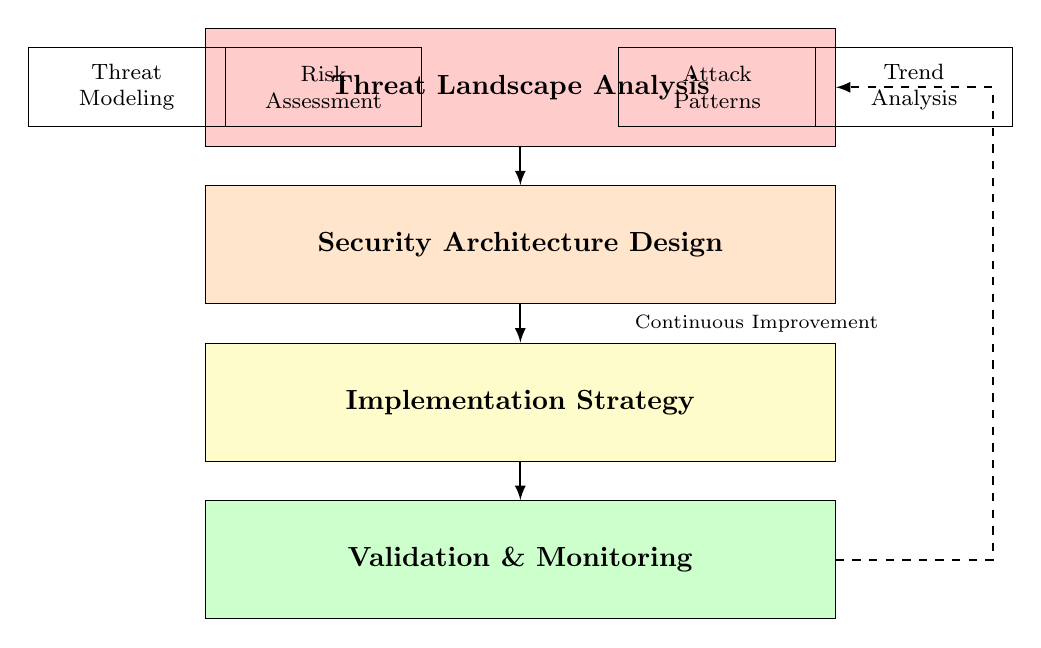
\begin{tikzpicture}[
    level/.style={rectangle, draw, text centered, minimum width=8cm, minimum height=1.5cm},
    component/.style={rectangle, draw, text centered, minimum width=2.5cm, minimum height=1cm, font=\footnotesize},
    arrow/.style={->, thick, >=latex}
]

% Livelli principali
\node[level, fill=red!20] (threat) at (0,0) {\textbf{Threat Landscape Analysis}};
\node[level, fill=orange!20] (arch) at (0,-2) {\textbf{Security Architecture Design}};
\node[level, fill=yellow!20] (impl) at (0,-4) {\textbf{Implementation Strategy}};
\node[level, fill=green!20] (valid) at (0,-6) {\textbf{Validation \& Monitoring}};

% Componenti
\node[component, align=center] (t1) at (-5,0) {Threat\\Modeling};

\node[component, align=center] (t2) at (-2.5,0) {Risk\\Assessment};
\node[component, align=center] (t3) at (2.5,0) {Attack\\Patterns};
\node[component, align=center] (t4) at (5,0) {Trend\\Analysis};

% Frecce di flusso
\draw[arrow] (threat) -- (arch);
\draw[arrow] (arch) -- (impl);
\draw[arrow] (impl) -- (valid);

% Feedback loop
\draw[arrow, dashed] (valid.east) -- ++(2,0) -- ++(0,6) -- (threat.east);
\node[font=\scriptsize] at (3,-3) {Continuous Improvement};

\end{tikzpicture}
\caption{Framework integrato di sicurezza GDO: dal threat landscape all'architettura}
\label{fig:framework_sicurezza}
\end{figure}

\end{document}
% --- IGNORE ---